\chapter{The carbon footprint of surgical and non-surgical skin cancer appointments}
\label{ch-6}
\begin{refsection}[refs/ch-6.bib]

The aim of this chapter was to estimate the carbon emissions of an appointment for dermoscopy guided full skin examination, total body photography, and the excision of a lesion suspicious for melanoma or other skin cancers for patients attending specialist dermatology clinics in Sydney, Australia. This chapter contains the same text as a manuscript currently being reviewed by \textit{Clinical and Experimental Dermatology}. Supplementary material are provided in Appendix \ref{ap-e}. A protocol was published on the \textit{Open Science Framework} and is provided in Appendix \ref{ap-f}.

\paragraph*{Publication details}
Manuscript authored by Jake T W Williams, Katy J L Bell, Rachael Morton, Pascale Guitera, Linda K Martin, and Scott McAlister. It was submitted to \textit{Clinical and Experimental Dermatology} and is currently under review.

\clearpage

\section{Abstract}

\subsection{Background}
The carbon emissions of the healthcare sector are large and there is a growing literature dedicated to estimating the carbon footprint of healthcare activities. The carbon footprint of dermatology services is of particular interest in Australia due to the high burden of melanoma and non-melanoma skin cancer and the geographically dispersed population.

\subsection{Objectives}
The goal of this study was to estimate the carbon emissions of an appointment for dermoscopy guided full skin examination, total body photography, and the excision of a lesion suspicious for melanoma or other skin cancers for patients attending specialist dermatology clinics in Sydney, Australia. 

\subsection{Methods}
The carbon footprint of each appointment type was estimated in kilograms carbon dioxide equivalent (CO2-e) using process-based life cycle assessment. We included patient transport, single-use equipment, reusable equipment requiring treatment, and energy. Each appointment type was investigated as a mutually exclusive event. 

\subsection{Results}
Total carbon emissions were 11.11 kg CO2-e (95\% CI 1.93 – 55.53) for a full skin examination, 10.75 kg CO2-e (95\% CI 1.60 – 54.54) for total body photography, and 12.21 kg CO2-e (95\% CI 2.92 – 61.58) for the excision of a lesion suspicious for melanoma. Patient transport was responsible for 10.72 kg CO2-e for each appointment type. 

\subsection{Conclusions}
Carbon emissions associated with dermoscopy guided full skin examination, total body photography, and the excision of a lesion suspicious for melanoma or other skin cancers were similar and largely driven by patient transport. Efforts to reduce emissions related to skin cancer care should focus on reducing the need for patients to attend the clinic, where it is clinically safe to do so. 

\section{Introduction}
Climate change is having devastating health impacts, including from the direct impact of heat and extreme weather events, and from the indirect impact of economic and societal changes.\cite{romanello_2024_2024} Climate change is caused by the increase of greenhouse gasses (GHG) in the atmosphere. The health sector is responsible for about 5\% of GHG emissions globally and between 5\% and 7\% of national emissions in Australia.\cite{lenzen_environmental_2020, malik_carbon_2018} Sustainable health systems have been endorsed in many countries,\cite{wise_cop26_2021} and there is increasing recognition of the need to reduce the GHG emissions of healthcare sectors.\cite{macneill_planetary_2021}

Life cycle assessment (LCA) is a method used to quantify the environmental impact of products and services, and it is increasingly being used to estimate the environmental impact of healthcare technologies and medical interventions.\cite{rasmussen_environmentally_2025, drew_healthcarelca_2025} Process-based LCA is a specific type of LCA that uses a bottom-up approach and granular information about material mass, energy use, transport, and other components of an intervention to model environmental impact. The alternative method, known as environmentally-extended input output analysis, uses financial data as its basis for estimation and is less accurate for LCAs of individual healthcare items and procedures.\cite{mcalister_how_2024}

The environmental impact of dermatology appointments is of particular interest in Australia given the high burden of melanoma and non-melanoma skin cancer and sometimes large geographical distances between where patients live and the nearest skin cancer clinic (dermatology clinic or skin-cancer trained GP clinic). Patients may attend clinics for different purposes related to skin cancer, for example for: melanoma and keratinocyte cancer surveillance, diagnostic processes, and surgical and non-surgical treatments. 

Full skin examinations typically involve physical examination and dermoscopy, a non-invasive technique using a dermatoscope (illuminated magnifying glass) to visualise features of the skin not visible to the naked eye. Sequential dermoscopic digital imaging describes digital (dermoscopic) photographs of lesions taken during these examinations to compare changes over time.\cite{adler_methods_2019} Total body photography is a related health service where images of the entire body are taken to act as a baseline and help detect changes to the skin.\cite{adler_methods_2019} Skin excisions are undertaken to remove lesions suspicious for skin cancer and common types include excisional biopsy, punch biopsy, or shave biopsy, performed according to suspected clinical diagnosis, lesion size, and body part. 

The goal of this study was to estimate the carbon emissions of an appointment for dermoscopy guided full skin examination, total body photography, and the excision of a lesion suspicious for melanoma or keratinocytic cancer. 

\section{Methods}

\subsection{Overview of methodology}

Life cycle assessment (LCA) is defined by international standards as the “compilation and evaluation of the inputs, outputs, and the potential environmental impacts of a product system throughout its life cycle”.\cite{international_organization_for_standardization_iso_2006} It is commonly used to estimate greenhouse gas emissions associated with the entire life cycle of a product system, from raw material extraction to final waste disposal. This study uses the methodology of an attributional process-based LCA to estimate the greenhouse gas emissions associated with different kinds of appointments to a skin cancer specialist dermatology clinic. It follows International Organisation for Standardisation (ISO) standards 14040:2016 and 14044:2016.\cite{international_organization_for_standardization_iso_2006, international_organization_for_standardization_iso_2006-1} The study’s aims and methods were pre-specified in a protocol registered on the Open Science Framework prior to any analysis being undertaken.\cite{williams_climate_2025}

\subsection{Study setting}

This study was conducted based on healthcare activities observed at two skin cancer focused subspeciality dermatology clinics in metropolitan Sydney, New South Wales, Australia: Sydney Melanoma Diagnostic Centre (SMDC) and Melanoma Dermatology (MD). SMDC is based at Royal Prince Alfred Hospital in Camperdown and MD is part of the Melanoma Institute Australia at the Poche Centre in Wollstonecraft. Ethical approval was not sought for the collection of data on healthcare activities. Data from the MELanoma SELF surveillance (MEL-SELF) trial was used to estimate emissions from patient transport. The MEL-SELF trial was approved by the Sydney Local Health District (RPAH zone) Ethics Review Committee (2019/ETH13612). Details of the trial are available elsewhere.\cite{ackermann_can_2021} 

\subsection{Study design}

This attributional process-based carbon footprint investigated three functional units related to the surveillance, and surgical excision of melanoma and keratinocytic cancers. The scheduled appointment of one patient for either: (1) a dermoscopy-guided full skin examination, (2) two-dimensional total body photography (excluding full skin examination), or (3) an excision of one or more lesions suspicious for melanoma or other skin cancers. 

The system boundary, which specifies the processes included in or excluded from the analysis, is provided in Figure \ref{fig:ch-6-fig-1}. This study included single-use disposable equipment, reusable equipment requiring sterilisation or washing between uses, patient travel, and general electricity use. It excluded reusable equipment that did not require any sterilisation or washing between uses, capital infrastructure, and pharmaceuticals on the basis that their greenhouse gas emissions per dermatology appointment were expected to be less than 1\% of the total emissions for that functional unit. Staff transport was excluded because it was not considered part of the functional units investigated in this study. For the excision functional unit, we only included processes that took place within the dermatology clinic and did not include the histopathological review of the lesion. 

\begin{figure}[p]
    \centering
    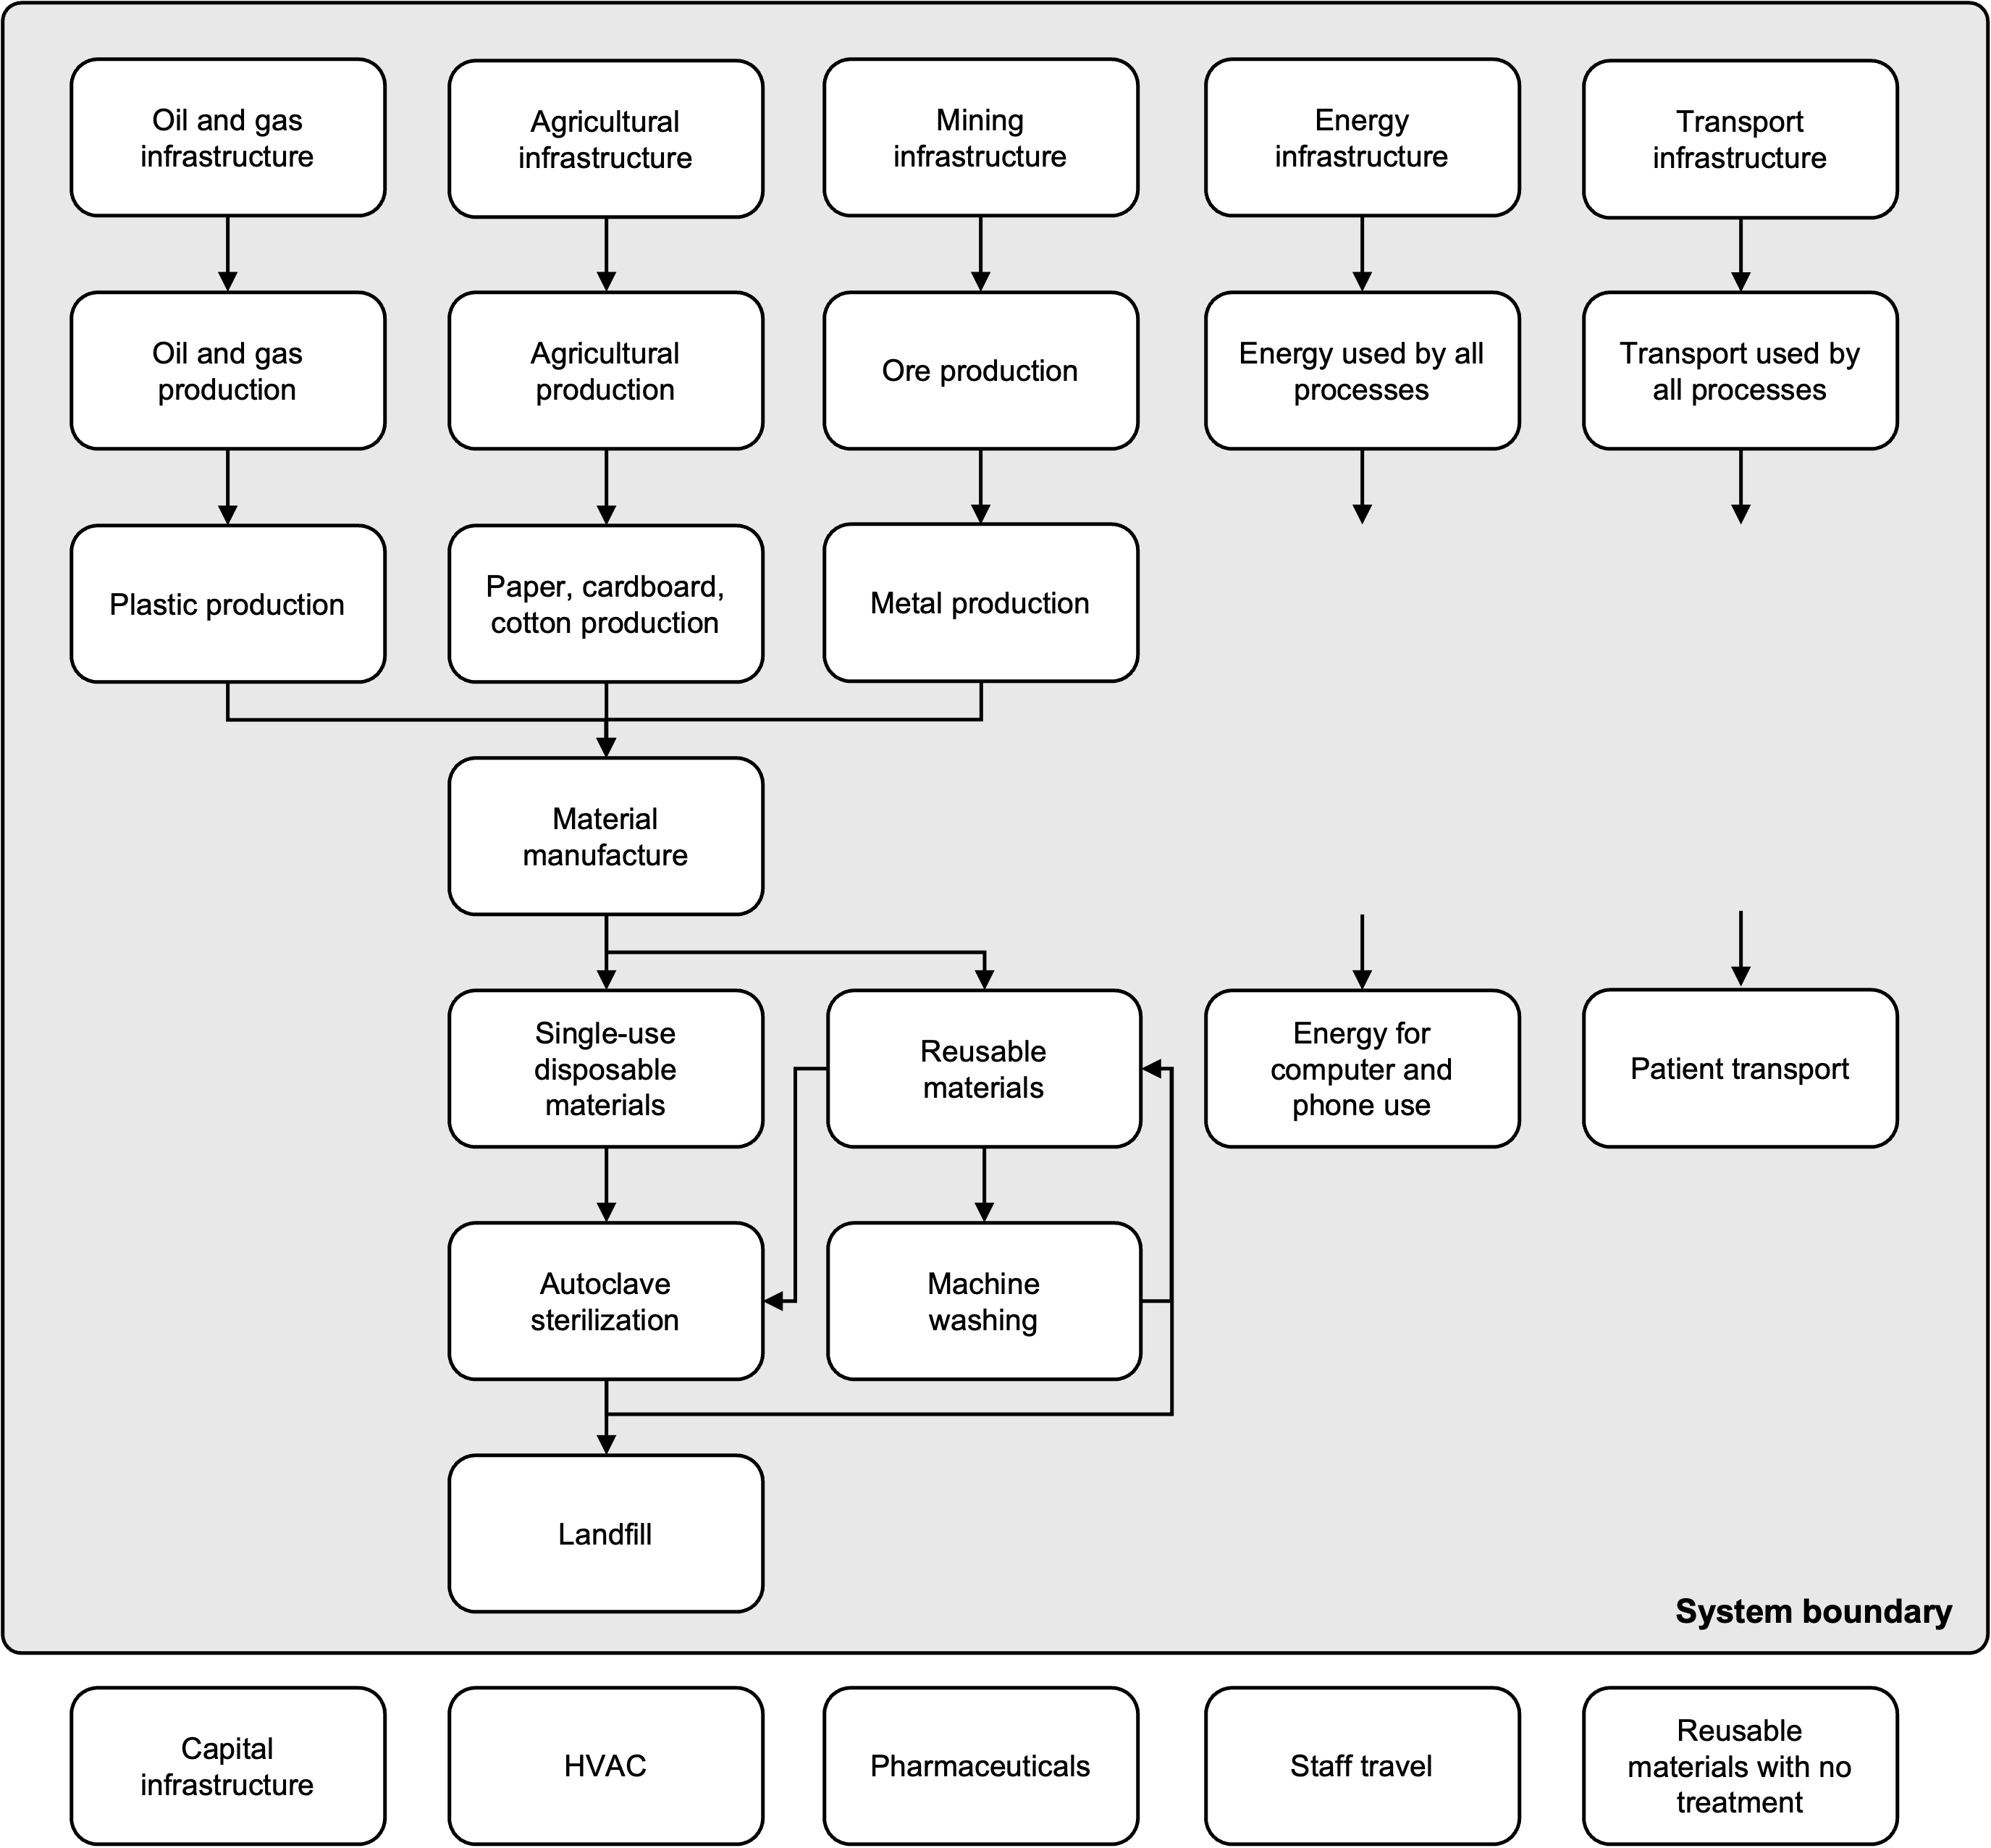
\includegraphics[width=1\linewidth]{core-chapters/figs/ch-6-fig-1.png}
    \caption{System boundary of the analysis.}
    \label{fig:ch-6-fig-1}
\end{figure}

\subsection{Study outcomes}
The primary outcome was greenhouse gas emissions in kilograms of carbon dioxide equivalent units (kg CO2-e). We included emissions from fossil, biogenic, and land use sources.

\subsection{Data collection}
Methods for data collection are provided in Supplementary Note 1. 

\subsection{Data analysis}
Data cleaning and analysis was conducted using R Version 4.4.3 and R Studio Version 2025. Life cycle assessment was modelled using SimaPro Analyst Release 9.6.0.1 (Pré Sustainability, Amersfoot, Netherlands). Background data on the environmental impact of processes were obtained from the AusLCI Version 2 (Lifecycles, Melbourne, Australia) database which uses background environmental data from Ecoinvent Version 3.10 (Ecoinvent, Zurich, Switzerland) databases. Impact assessment was modelled using the “IPCC 2021 GWP100” method (Version 1.03). Details and assumptions of modelling in SimaPro are provided in Supplementary Table 2. The primary outcome was reported for the entire functional unit, as well as for single use materials, reusable materials, electricity use, and patient travel.

\subsection{Subgroup analysis}
We undertook two subgroup analyses for emissions associated with appointments for surgical procedures. For the first, we compared emissions associated with the three types of surgical procedure for one lesion: excision, shave biopsy, and punch biopsy. For the second, we compared emissions for excision of one lesion versus multiple lesions during the same appointment. 

\subsection{Sensitivity analysis}
We conducted sensitivity analyses to determine the impact of different methods used to estimate patient travel (Supplementary Note 1). First, we excluded patients who travelled by plane to understand the impact of low-frequency but high-emission transport (details are provided in Supplementary Table 1). Second, transport emissions were halved to account for travel to two destinations on the same journey (e.g., if the patient drove to the clinic, had their appointment, went shopping, then went home). 

We conducted Monte Carlo simulations using 1,000 runs for all primary and subgroup analyses to estimate 95\% confidence intervals for greenhouse gas emissions. Monte Carlo simulation, conducted in SimaPro, uses random values within the probability distributions of inputs and outputs of all processes used in the study. We included all materials in this analysis, including those used during less than 50\% of observed appointments. Probability distributions of likely values for the number of materials used per appointment (single use and reusable), patient distance travelled, and appointment duration were modelled using either a triangular or log normal distribution. For triangular distributions, possible values were assumed to be between the minimum and maximum observed value. The most likely value was assumed to be the median. 

\section{Results}
Data collection by clinic is reported in Supplementary Table 3. Appointment length is reported in Supplementary Table 4. Material use is reported in Supplementary Tables 5-7 and materials included in the primary analysis are listed in Table 1. Details about the number and type of excisions performed during the excision appoints is reported in Supplementary Table 8. Material composition and weight is provided in Supplementary Table 9. Patient travel distance and mode of transport is reported in Supplementary Table 1. Material use for subgroup analyses are reported in Supplementary Tables 10-13. Material use for sensitivity analyses are reported in Supplementary Tables 1, 4, 5-7, 10, 12.

Greenhouse gas emissions associated with each functional unit are reported in Table 2. In all three functional units, patient transport was responsible for 10.72 kg CO2-e and was the greatest contributor to the total emissions (96\% for full skin examination, >99\% for total body photography, and 88\% for an excision of a lesion suspicious for melanoma) (Figure \ref{fig:ch-6-fig-2}). Total emissions were 11.11 kg CO2-e for a full skin examination, 10.75 kg CO2-e for total body photography, and 12.21 kg CO2-e for an excision of a lesion suspicious for melanoma. Emissions from single-use materials reflect the number and type of items included in the analysis (Table 1). For total body photography only single-use paper towels were included, and emissions were relatively low (0.01 kg CO2-e). For excisions, 18 single-use (e.g., gauze, suture, gloves) and four reusable (e.g., scissors, needle holder, scalpel handle) materials were included, and emissions were relatively high (1.26 kg CO2-e). Emissions from energy use was low across all three functional units. 

\begin{figure}
    \centering
    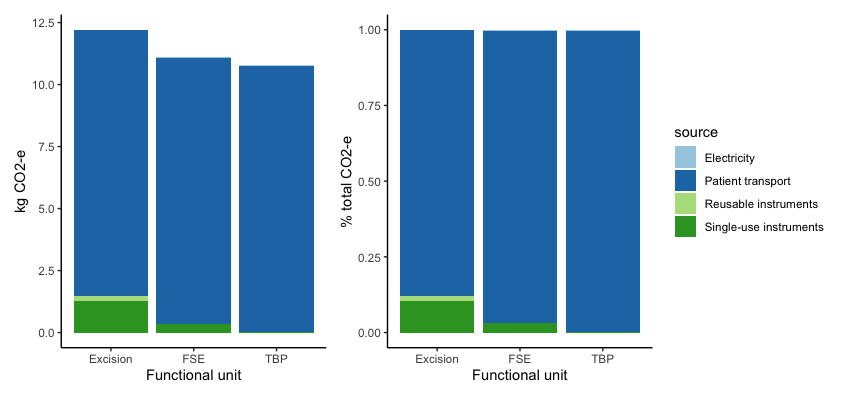
\includegraphics[width=1\linewidth]{core-chapters/figs/ch-6-fig-2.png}
    \caption{Greenhouse gas emissions of full skin examination, total body photography, and excision of a lesion suspicious for melanoma, by source of emission.}
    \label{fig:ch-6-fig-2}
\end{figure}

Subgroup analyses found slightly lower total emissions for shave biopsy than other excision types (12.20 kg CO2-e for one excision biopsy, 13.65 kg CO2-e for one punch biopsy, and 11.36 kg CO2-e for one shave biopsy), and a modest increase for >1 concurrent excisions (11.72 kg CO2-e for one lesion and 12.43 kg CO2-e for more than one lesion). These differences were largely explained by variation in emissions from single use instruments between subgroups. These were higher for excision biopsies (1.25 kg CO2-e) than for punch (0.97 kg CO2-e) and shave (0.64 kg CO2-e) biopsies, and for appointments with more than one lesion removed (1.48 kg CO2-e) than for appointments with only one lesion removed (0.82 kg CO2-e). Details are reported in Supplementary Table 14. 

Sensitivity analyses found emissions from patient travel reduced from 10.72 to 9.69 kg CO2-e when travel by plane was excluded (n=2/262; 0.8\%), and to 5.36 kg CO2-e when an additional destination was assumed to occur on the dermatology clinic journey. Emissions reduced to 4.85 kg CO2-e when both were true (i.e., plane travel was excluded and an additional destination was assumed to occur on the journey). The results of the primary analysis were highly sensitive to the methods used to calculate emissions from patient transport.

Monte Carlo simulations showed large uncertainties. Confidence intervals (95\%) for total GHG emissions (kg CO2-e) were 1.93 – 55.53 for full skin examination, 1.60 – 54.54 for total body photography, and 2.92 – 61.58 for excision. Probability distributions of the Monte Carlo simulations were skewed and followed a log normal pattern. Full results of Monte Carlo simulations are reported in Supplementary Table 15.

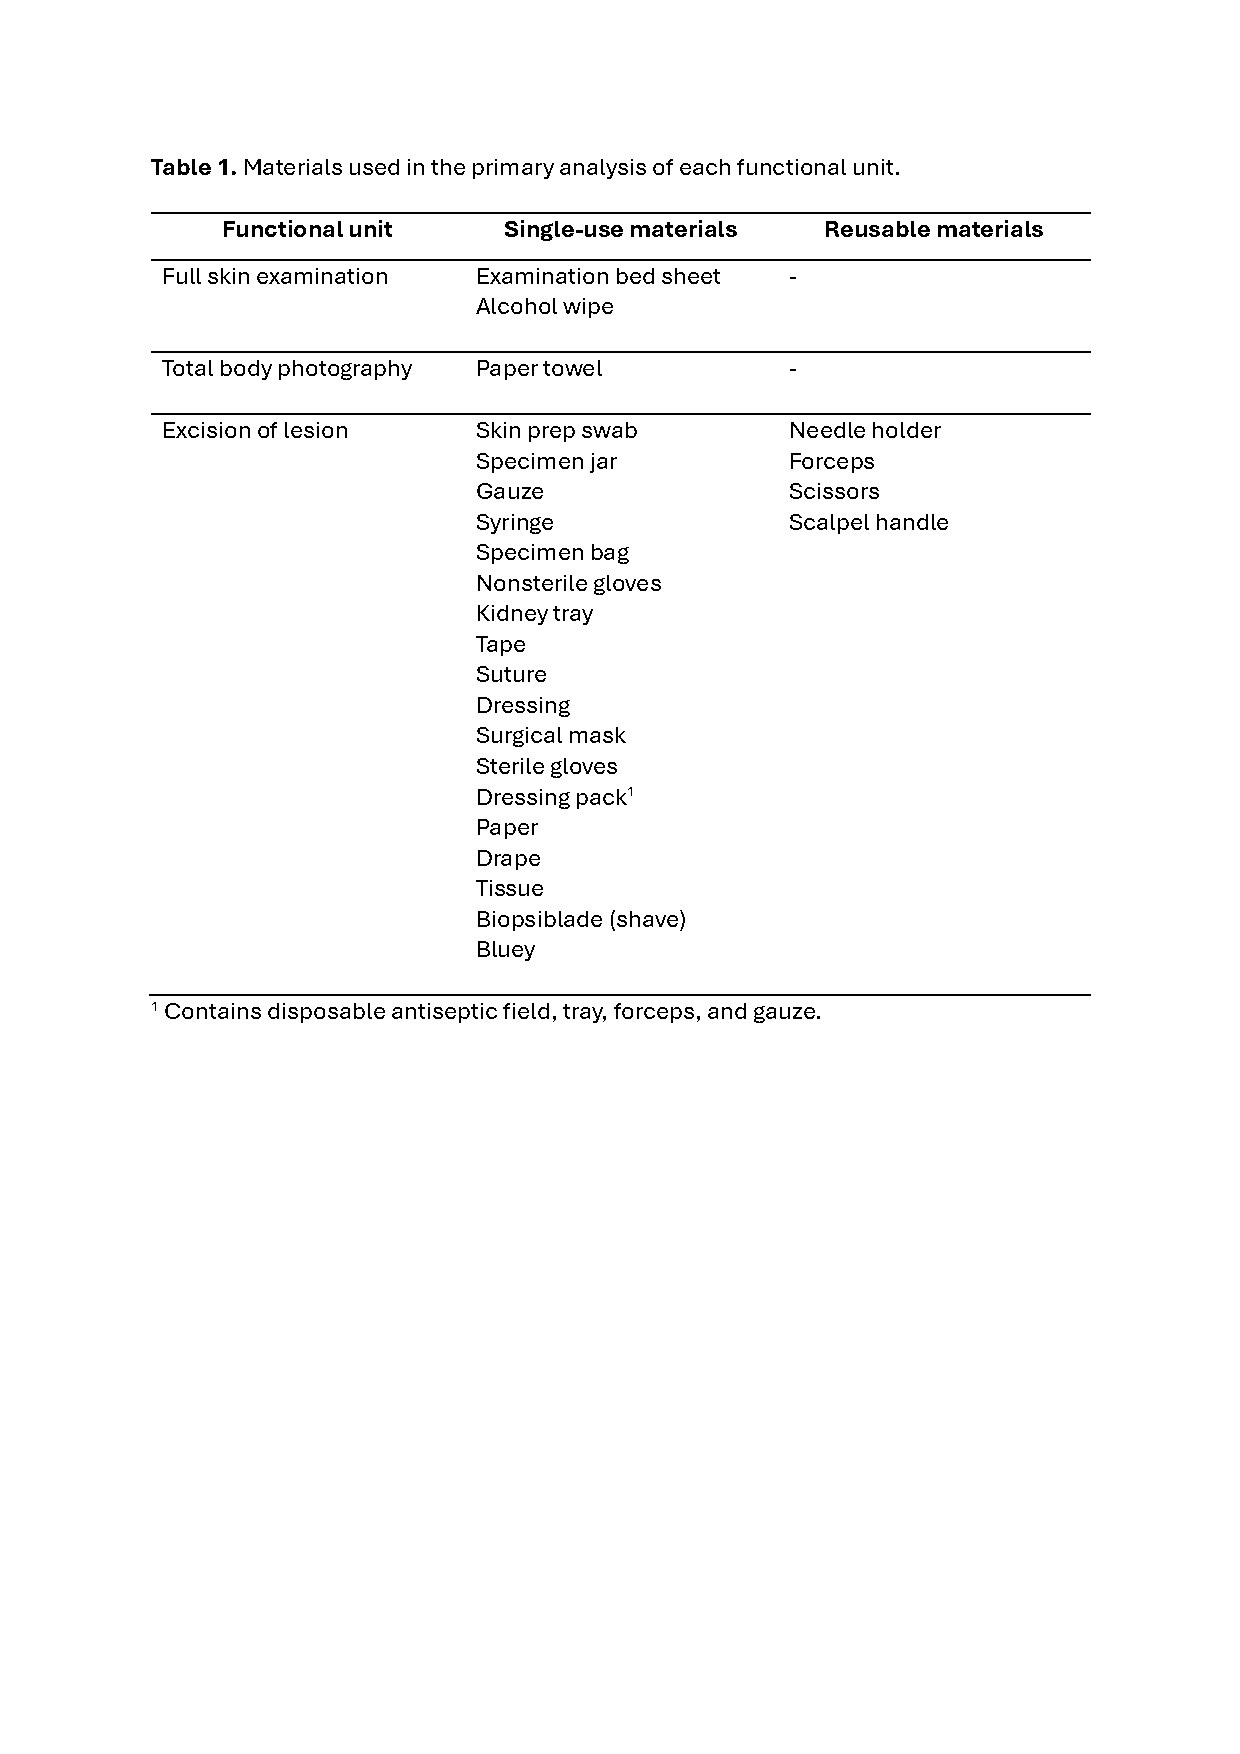
\includepdf[]{core-chapters/ch-6-tab-1.pdf}
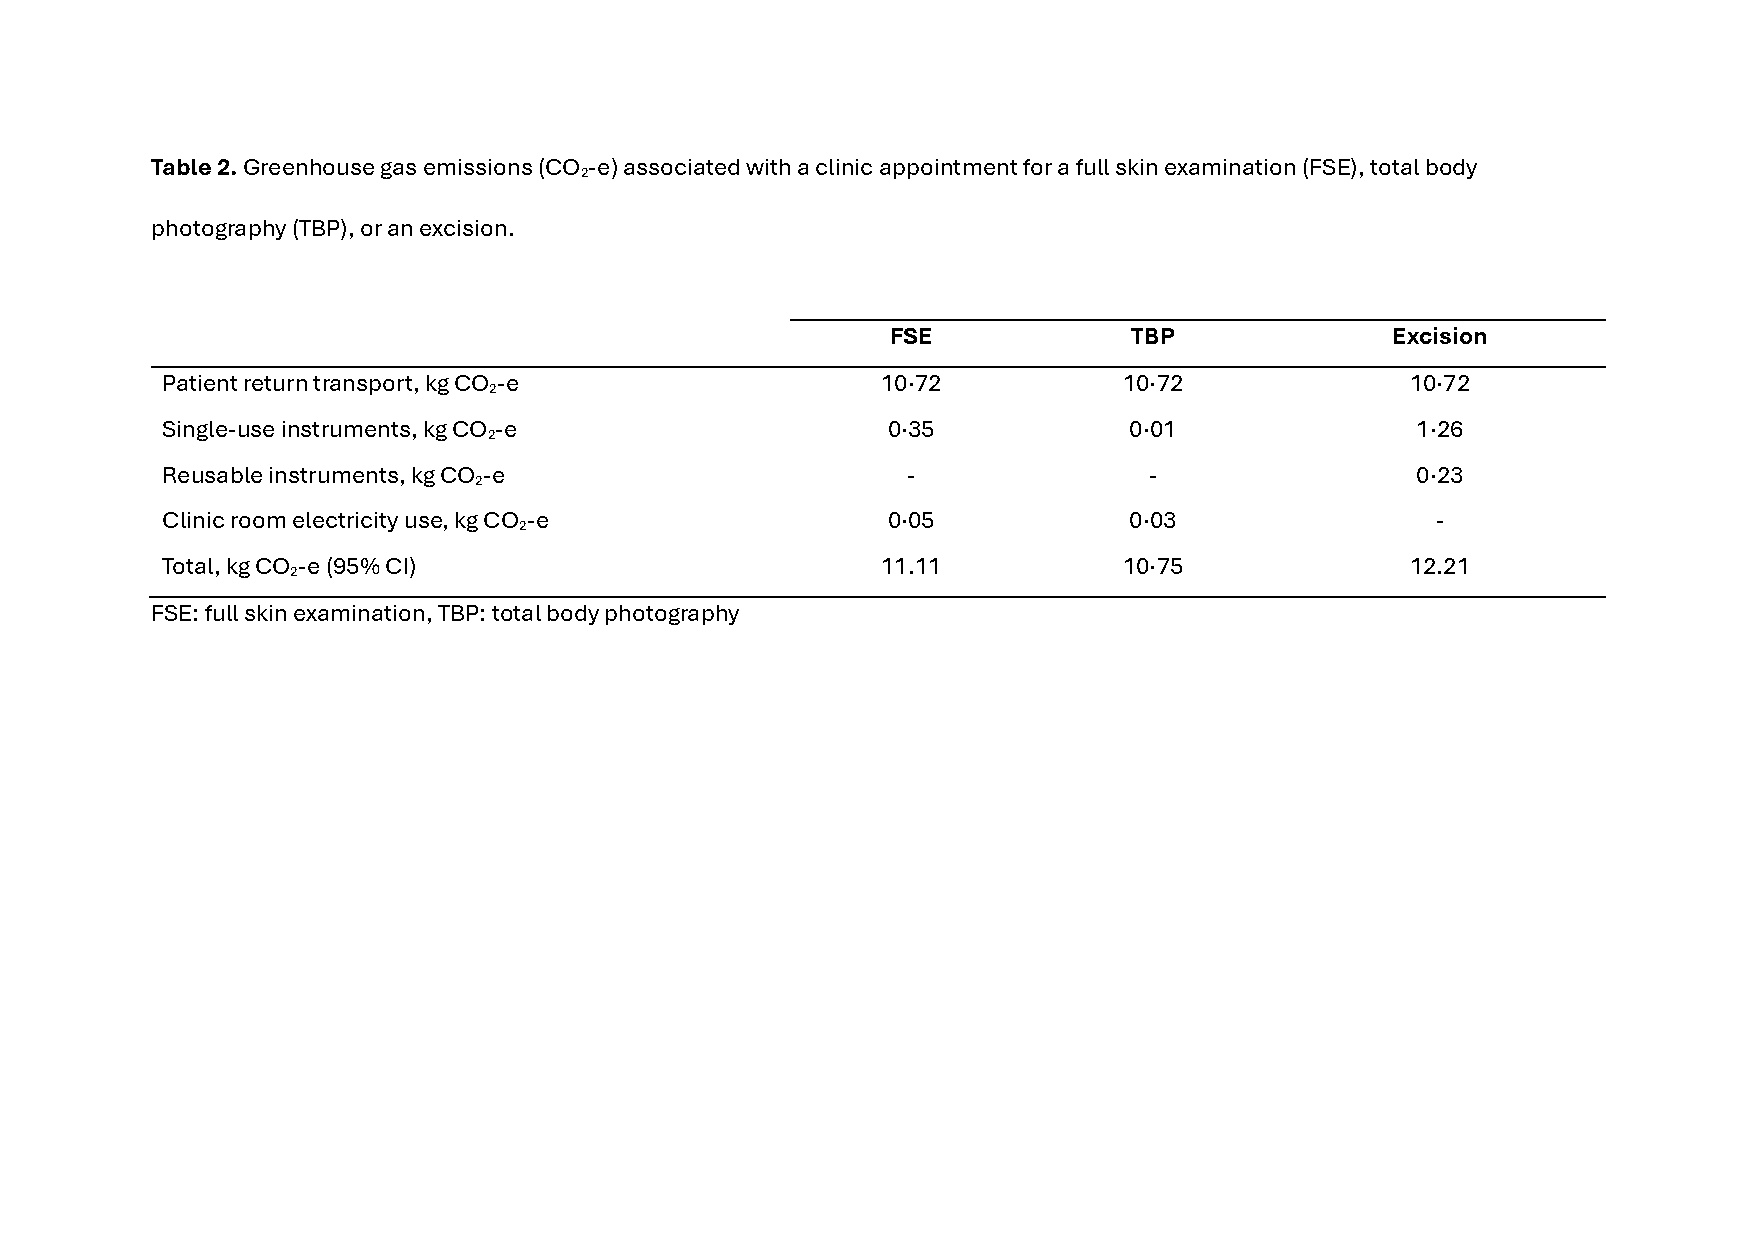
\includepdf[landscape=true]{core-chapters/ch-6-tab-2.pdf}

\section{Discussion}

This study reports the carbon emissions associated with an appointment for a full skin examination, total body photography, and an excision of a lesion suspicious for skin cancer. Emissions were similar between the three activities and ranged between 10.75 kg and 12.21 kg CO2-e. Among surgical appointments, total emissions were similar for different types of procedure (excision biopsy, punch biopsy, shave biopsy) and for the number of lesions removed in a single appointment (one lesion, more than one lesion). 

In all three functional units carbon emissions were driven by patient transport, which accounted for 88\% to more than 99\% of emissions in the primary analyses. Single-use and reusable materials accounted for less than 1\% of total emissions in the non-surgical functional units and 13\% in the surgical functional unit, reflecting the higher number of materials used during excisions of the skin than in full skin examinations and total body photography. Monte Carlo simulations suggest the findings of this study are uncertain with point estimates having large confidence intervals. Still, it highlights the importance of patient transport as a key component of the carbon emissions associated with clinical dermatology care. Patient transport is likely to be important for clinical appointments for other conditions in which a small number of materials are consumed, such as non-surgical general practice or specialist consultations. Our findings are consistent with those from a recent review that, when included, patient travel has relatively large contributions to the carbon emissions of hospital services and care pathways.\cite{kouwenberg_carbon_2024}

Only a few studies have investigated the carbon emissions of skin cancer dermatology care globally. Recent studies estimated the annual emissions of a large dermatology practice in the United States (324 t CO2-e per year)\cite{silva_carbon_2025} and emissions for different melanoma follow-up guidelines in the United Kingdom (ranging between 166 kg and 316 kg CO2-e per person per year).\cite{grover_relative_2024} Another study estimated emissions of hypothetical virtual compared to in-person review of a skin lesion in Aotearoa New Zealand, reporting 11 kg CO2-e fewer emissions per appointment in hypothetical virtual follow-up.\cite{jones_virtual_2024} These studies provide some context to our results but are not based on the findings of full process-based life cycles assessments. As with all studies of carbon emissions, the conclusions drawn depend on the scope of the analysis. For example, in the US study by Silva et al. purchased goods and services were the dominant source of emissions,\cite{silva_carbon_2025} whereas in our analysis patient transport dominated the results.

There are two existing process-based LCA in this field, one for the surgical removal of a skin cancer in a dermatology clinic in Australia and one for non-melanoma skin cancer surgery in a specialist plastic surgery centre in Wales.\cite{tan_carbon_2021, ang_carbon_2024} 

The Australian study, by Tan \& Lim, reports carbon emissions of 29 kg CO2-e per excision, approximately triple our finding but within our 95\% confidence interval estimate for this functional unit (2.92 – 61.58 kg CO2-e per appointment). This difference is partly attributable to differences in system boundaries and modelling assumptions between the two studies. This is common in life cycle assessment research. Notably, Tan \& Lim included staff travel within their system boundary, which was excluded from this study, and empirical data for mode of transport and distance travelled was not used. Another difference relates to the transportation of materials to and from the clinic. Tan \& Lim estimate this to be about 8.6 kg CO2-e per appointment, compared to our estimate of 1.5 kg CO2-e for total emissions from the full material life cycle (including transportation to and from the clinic and all other stages of the life cycle). The drivers of this difference are difficult to determine with certainty. One possible explanation is a difference in the way emissions from transport of materials to and from the clinic were included. Specifically, whether emissions were included based on the total vehicle distance travelled (e.g., emissions per kilometre), or on the proportion of those emissions attributable to the weight of the relevant items carried by that vehicle (e.g., emissions per gram-kilometre), which was often only a few grams per item (see Supplementary Table 7).

It is important to note that the scenarios investigated in this study are not substitutable and have different purposes. A full skin examination has a different purpose to an excision of a lesion or total body photography, and emissions reductions cannot be estimated between the functional units. Even within the surgical functional unit, clinical practice guidelines recommend the use of excision, punch, and shave biopsies for different purposes, and while emissions may be (non-significantly) lower for shave excisions, it would be incorrect to recommend this procedure in the context of a lesion suspicious for melanoma.\cite{adler_methods_2019}

Despite this, there are opportunities for clinical practice to reduce carbon emissions based on the findings of this study. An existing review of sustainable dermatological surgery made several recommendations to reduce emissions, and these should be implemented where it is safe to do so.\cite{ali_environmental_2025, ali_environmental_2025-1} The findings of this study suggest that most emissions from clinic appointments are attributable to patient transport and therefore reducing the need for this transport will have the greatest impact. Previous studies of emissions from healthcare services have therefore encouraged the use of carpooling, public transport, and cycling in an effort to reduce these emissions.\cite{tan_carbon_2021, barraclough_carbon_2025} Emissions from patient transport can also be reduced by performing multiple procedures or investigations on the same day wherever clinically acceptable, for example by performing a full skin examination and an excision during the same visit instead of in two separate visits. This reduces emissions from 23.32 to 12.6 kg CO2-e (Table 1). While all these actions may be effective, clinicians seeking to reduce emissions should focus on reducing the need for patients to visit the clinic in the first place where this is clinically appropriate, such as by reducing unnecessary excisions and appointments.

Healthcare overuse is a well described problem in modern medicine and is associated with harms to the patient, practitioner, public, and planet.\cite{gram_less_2025} These harms include carbon emissions, such as those described in this study, which are emitted without any health benefit to the patient.\cite{barratt_high_2022} While the issue of overdiagnosis was not explored directly in this study, previous work suggests that the overdiagnosis of melanoma may be common, especially for in-situ melanoma in patients who have had full skin examinations, which results in cascades of subsequent care and a higher rate of healthcare use and environmental impacts with no health benefit to the patient.\cite{bell_melanoma_2022} Some full skin examinations, total body photographs, or excisions are likely unnecessary, and limiting these is an effective way to reduce emissions. This could include tailoring services according to need by adopting a risk-based approach to screening and surveillance (FSE and TBP) and using new technologies to monitor lesions and reduce unnecessary skin excisions,\cite{pellacani_effect_2022, smith_implementing_2024} including the possibility of remote monitoring.\cite{drabarek_perspectives_2022} This is of particular importance in Australia given the recently announced roadmap for a targeted national skin cancer screening program, and its equity objectives of providing access to screening regardless of where a person lives.

This study has several strengths. First, we used process-based life cycle assessment methodology to estimate carbon emissions across the entire life cycle of all processes included in this study. Process-based LCAs are the most accurate way to estimate carbon emissions at the level of a single healthcare activity. Second, we collected and used empirical data about materials and patient transport and did not rely on estimates for these parts of our analysis. This is especially beneficial for patient transport because it accounted for such a large proportion of emissions. Previous studies made assumptions about distance travelled and modality of transport.\cite{tan_carbon_2021}

The primary limitation of this study is that it is based on data collected from two Australian metropolitan specialist clinics in Sydney and this is likely to impact on the distance travelled and modality of transport used by patients. This means our findings may not be applicable to other parts of Australia, particularly regional and small community practices where transportation is likely to be very different. It may also not be applicable to some international contexts with higher proportions of patients using public transport and smaller distances for those who drive. Parts of our model are based on assumptions and data that was not directly measured. This included assuming shipping and road-transport distances from the manufacturer of materials to the clinic, and transport from the clinic to sterilisation and landfill sites. We also excluded several processes on the basis that their emissions were likely to contribute less than 1\% of emissions. Emissions from the pathological review of excised skin lesions was excluded, as were emissions from all the cascaded care that follows a melanoma diagnosis.

This study found carbon emissions associated with dermoscopy-guided full skin examination, total body photography, and the excision of a lesion suspicious for melanoma or keratinocytic cancer were similar and almost exclusively driven by patient transport. Emissions reductions can be achieved by reducing the need for patients to visit the clinic, where this is safe to do so.


\printbibliography[heading=subbibliography]
\end{refsection}
